%!TEX program = xelatex
\documentclass[aspectratio=169, xcolor=table]{beamer}
\usepackage[UTF8]{ctex} % Use default font set
\usepackage{hyperref}

% other packages
\usepackage{latexsym,amsmath,xcolor,multicol,booktabs,calligra}
%\usepackage[table]{xcolor}
\usepackage{siunitx} % For \SI command
\usepackage{graphicx,pstricks,listings,stackengine}
\usepackage{tikz}
\usetikzlibrary{patterns}
\usetikzlibrary{shadows}
\usetikzlibrary{snakes}
\usetikzlibrary{decorations.pathmorphing}
\usepackage{tikz-3dplot}
\usepackage{fontawesome5}
\usepackage{bm}

\author{Yu Shu \& Chihao Shi}
\title{力学A(PHYS1001A.04):狭义相对论部分习题课}
\subtitle{Course NOT easy: Time is Relative, but your Grade is Absolute.}
\institute{School of Physics, USTC}
\date{Jan.7, 2026}
\usepackage{USTC} 

% defs
\def\cmd#1{\texttt{\color{red}\footnotesize $\backslash$#1}}
\def\env#1{\texttt{\color{blue}\footnotesize #1}}
\definecolor{deepblue}{rgb}{0,0,0.5}
\definecolor{deepred}{rgb}{0.6,0,0}
\definecolor{deepgreen}{rgb}{0,0.5,0}
\definecolor{halfgray}{gray}{0.55}

\lstset{
    basicstyle=\ttfamily\small,
    keywordstyle=\bfseries\color{deepblue},
    emphstyle=\ttfamily\color{deepred},    % Custom highlighting style
    stringstyle=\color{deepgreen},
    numbers=left,
    numberstyle=\small\color{halfgray},
    rulesepcolor=\color{red!20!green!20!blue!20},
    frame=shadowbox,
}

\begin{document}

\begin{frame}
    \titlepage
    \begin{figure}[htpb]
        \begin{center}
            \includegraphics[width=0.15\linewidth]{pic/ustc_logo_fig-eps-converted-to.pdf}
        \end{center}
    \end{figure}
\end{frame}

\begin{frame}
    \tableofcontents[sectionstyle=show,subsectionstyle=show/shaded/hide,subsubsectionstyle=show/shaded/hide]
\end{frame}

\section{内容回顾与补充拓展}

\subsection{物理直觉的重塑}

\begin{frame}[shrink=5]
    \begin{columns}[T] % 顶部对齐
        \column{0.48\textwidth}
            \footnotesize % 全栏缩小字号
            \begin{block}{1. 牛顿-伽利略变换}
                经典速度合成遵循矢量加法:
                \begin{equation}
                    \vec{v}_{AB} = \vec{v}_A - \vec{v}_B \implies c' = c \pm v
                \end{equation}
                \textbf{推论}:若光是波,波速 $c$ 必依赖于“以太”和观测者的运动。
            \end{block}

            \begin{block}{2. 麦克斯韦方程组的挑战}
                麦克斯韦方程组导出的光速:
                \begin{equation}
                    c = \frac{1}{\sqrt{\epsilon_0 \mu_0}} \approx 3 \times 10^8 \text{m/s}
                \end{equation}
                \textbf{矛盾}:此公式中\textbf{无参考系项}!
                \\ \alert{问题:$c$ 到底是相对于谁的速度?}
            \end{block}

        \column{0.48\textwidth}
            \footnotesize % 全栏缩小字号
            \begin{alertblock}{3. 历史的判决:M-M 实验}
                迈克尔逊-莫雷实验试图探测地球相对于“以太”的运动(以太风)。
                \begin{itemize}
                    \item \textbf{预期}:干涉条纹随旋转移动。
                    \item \textbf{结果}:\textbf{零结果 (Null Result)}。
                \end{itemize}
            \end{alertblock}

            \vspace{0.2em}
            \centering
            % 紧凑版 M-M Experiment Diagram
            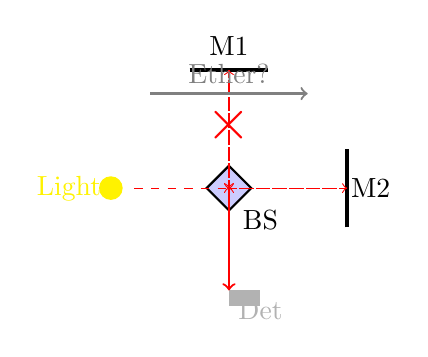
\begin{tikzpicture}[scale=1, every node/.style={transform shape}]
                % Beam Splitter
                \draw[thick, fill=blue!20, rotate=45] (-0.2,-0.2) rectangle (0.2,0.2);
                \node at (0.4, -0.4) {BS};

                % Mirrors (更加紧凑的布局)
                \draw[ultra thick] (-0.5, 1.5) -- (0.5, 1.5); % Top M1
                \node at (0, 1.8) {M1};
                \draw[ultra thick] (1.5, -0.5) -- (1.5, 0.5); % Right M2
                \node at (1.8, 0) {M2};

                % Source & Detector
                \fill[yellow] (-1.5, 0) circle (0.15) node[left] {Light};
                \fill[black!30] (0, -1.5) rectangle (0.4, -1.3) node[below] {Det};

                % Light Paths
                \draw[->, red, dashed] (-1.2, 0) -- (0, 0); % In
                \draw[->, red, dashed] (0, 0) -- (0, 1.5); % Up
                \draw[->, red, dashed] (0, 1.5) -- (0, 0); % Down
                \draw[->, red, dashed] (0, 0) -- (1.5, 0); % Right
                \draw[->, red, dashed] (1.5, 0) -- (0, 0); % Left
                \draw[->, red, thick] (0, 0) -- (0, -1.3); % Out
                
                % Ether Wind Arrow
                \draw[->, gray, thick] (-1, 1.2) -- (1, 1.2) node[midway, above] {Ether?};
                \node[red, font=\huge] at (0, 0.8) {$\times$};
            \end{tikzpicture}
            
            \vspace{0.1em}
            \scriptsize{\textbf{结论}:不存在以太风,光速各向同性。}
    \end{columns}
\end{frame}

\begin{frame}[shrink=5]{狭义相对论的逻辑基石:两大假设}
    \begin{columns}[T]
        \column{0.48\textwidth}
            \footnotesize
            \begin{block}{1. 相对性原理 (Principle of Relativity)}
                \textbf{内容}:所有物理定律(不仅是力学,包含电磁学)在所有惯性系中形式相同。
                \begin{itemize}
                    \item \textbf{推论}:没有优越的“绝对静止系”(以太不存在)。
                    \item \textbf{意义}:你无法通过任何内部实验(包括测光速)判断自己是静止还是匀速直线运动。
                \end{itemize}
            \end{block}

            \begin{block}{2. 光速不变原理 (Constancy of $c$)}
                \textbf{内容}:真空中的光速 $c$ 对任何惯性系观测者都是恒定值。
                \begin{equation}
                    c \approx 3 \times 10^8 \text{m/s}
                \end{equation}
                \textbf{核心}:与光源的运动状态\textbf{无关},与观测者的运动状态\textbf{无关}。
            \end{block}

        \column{0.48\textwidth}
            \footnotesize
            \begin{alertblock}{Survival Tip: 代价是什么?}
                如果速度 $c = \Delta x / \Delta t$ 恒定,而不同参考系看到的同一过程 $\Delta x$ 可能不同,那么 **$\Delta t$ (时间) 必须随之改变**!
                \\ $\implies$ \textbf{绝对时空观崩塌,时空耦合。}
            \end{alertblock}

            \vspace{0.5em}
            \centering
            \begin{tikzpicture}[scale=0.8]
                % Case 1: Classical Ball
                \node[anchor=west] at (-0.5, 2.2) {\textbf{A. 扔球 (经典)}};
                \draw[thick, fill=gray!20] (0, 1.5) rectangle (1.5, 2.0); % Train
                \node at (0.75, 1.75) {\tiny Train $v$};
                \draw[->, thick] (1.5, 1.75) -- (2.0, 1.75); % v vector
                
                \draw[->, blue, thick] (1.0, 2.0) -- (2.0, 2.5) node[right]{\tiny $u_{ball} = v + u'$};
                \fill[blue] (1.0, 2.0) circle (0.08);

                % Case 2: Relativistic Light
                \node[anchor=west] at (-0.5, 0.8) {\textbf{B. 射光 (相对论)}};
                \draw[thick, fill=gray!20] (0, 0) rectangle (1.5, 0.5); % Train
                \node at (0.75, 0.25) {\tiny Train $v$};
                \draw[->, thick] (1.5, 0.25) -- (2.0, 0.25);
                
                \draw[->, red, ultra thick, decorate, decoration={snake, amplitude=1pt, segment length=3pt}] (1.5, 0.25) -- (3.0, 0.25) node[right]{\tiny $c$ (NOT $c+v$)};
                
                % Ground Observer
                \draw[thick] (-0.5, -0.2) -- (3.5, -0.2);
                \node at (1.5, -0.5) {\tiny Ground Observer};
            \end{tikzpicture}
            
            \vspace{0.2em}
            \scriptsize{光速 $c$ 是宇宙速度的“硬上限”与“不变量”。}
    \end{columns}
\end{frame}

\begin{frame}[shrink=5]{同时的相对性}
    \begin{columns}[T]
        \column{0.48\textwidth}
            \footnotesize
            \begin{block}{思想实验:爱因斯坦的火车}
                设一列火车以速度 $v$ 向右运动,光源 $S'$ 位于车厢正中央。
                \begin{itemize}
                    \item \textbf{车上观测者 ($S'$)}:
                    光源在中央,光速恒定 $\implies$ 光\textbf{同时}到达车头 (A) 和车尾 (B)。
                    $$ t'_A = t'_B $$
                    \item \textbf{地面观测者 ($S$)}:
                    车尾 (B) 迎着光运动,车头 (A) 背着光运动。
                    $$ \text{路程关系:} d_B < d_A $$
                    $$ \text{结论:} t_B < t_A \text{ (光先到车尾)} $$
                \end{itemize}
            \end{block}

        \column{0.48\textwidth}
            \footnotesize
            \begin{alertblock}{结论:同时是相对的}
                \textbf{“在 $S'$ 系同时发生的异地事件,在 $S$ 系看不再同时。”}
                \begin{itemize}
                    \item 这不是视觉错觉,而是真实的物理测量结果。
                    \item 只有当两个事件在\textbf{同一地点}发生时,其同时性才是绝对的。
                \end{itemize}
            \end{alertblock}

            \vspace{0.5em}
            \centering
            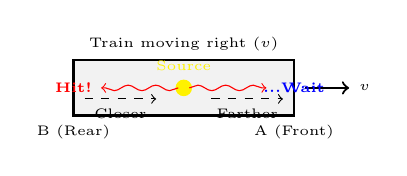
\begin{tikzpicture}[scale=0.7]
                % Ground View
                \draw[thick, fill=gray!10] (0,0) rectangle (4,1);
                \node at (2, 1.3) {\tiny Train moving right ($v$)};
                \draw[->, thick] (4.2, 0.5) -- (5, 0.5) node[right]{\tiny $v$};
                
                % Light Source
                \fill[yellow] (2, 0.5) circle (0.15) node[above=0.1cm]{\tiny Source};
                
                % Light Rays
                \draw[->, red, snake=snake, segment amplitude=1pt] (1.9, 0.5) -- (0.5, 0.5); % To Rear
                \draw[->, red, snake=snake, segment amplitude=1pt] (2.1, 0.5) -- (3.5, 0.5); % To Front
                
                % Events
                \node[red] at (0, 0.5) {\textbf{\tiny Hit!}};
                \node[blue] at (4, 0.5) {\textbf{\tiny ...Wait}};
                
                \node at (0, -0.3) {\tiny B (Rear)};
                \node at (4, -0.3) {\tiny A (Front)};
                
                % Logic Arrow
                \draw[->, dashed] (0.2, 0.3) -- (1.5, 0.3) node[midway, below]{\tiny Closer};
                \draw[->, dashed] (2.5, 0.3) -- (3.8, 0.3) node[midway, below]{\tiny Farther};
            \end{tikzpicture}
            
            \vspace{0.2em}
            \scriptsize{\textbf{地面视角}:车尾主动“撞”向光,车头在“躲”光。}
    \end{columns}
\end{frame}

\begin{frame}[shrink=10]{同时的相对性}
    \begin{columns}[T]
        \column{0.42\textwidth} % 左栏略窄,放公式
            \footnotesize
            \begin{block}{1. 坐标差变换公式}
                考虑在 $S$ 系中\textbf{同时}发生的两个事件 ($\Delta t = 0$),相距 $\Delta x$。
                代入 Lorentz 变换:
                \begin{equation}
                    \Delta t' = \gamma (\underbrace{\Delta t}_{0} - \frac{v}{c^2} \Delta x) = -\frac{\gamma v}{c^2} \Delta x
                \end{equation}
            \end{block}

            \begin{block}{2. 物理意义解析}
                \textbf{符号法则}:
                \begin{itemize}
                    \item 设 $v > 0$ (向右运动)。
                    \item 若 $\Delta x > 0$ (事件2在事件1的前方)。
                    \item 则 $\Delta t' < 0$ (事件2的时间坐标小于事件1)。
                \end{itemize}
                \textbf{结论}:空间上靠前的事件,时间上反而更早发生。
            \end{block}

        \column{0.56\textwidth} % 右栏加宽,放图和结论
            \small
            \begin{alertblock}{Survival Tip: “后方先发”判据}
                在运动参考系中观测,沿运动方向:
                \begin{itemize}
                    \item \textbf{后方 (Rear)} 的事件 \alert{\textbf{先发生 (Earlier)}}。
                    \item \textbf{前方 (Front)} 的事件 \alert{\textbf{后发生 (Later)}}。
                \end{itemize}
                \textit{口诀:船尾先闪,船头后亮。}
            \end{alertblock}

            \vspace{0.8em}
            \centering
            % 强化版时序图
            \begin{tikzpicture}[scale=1.5, every node/.style={transform shape}]
                % S' 系(飞船/滑块)
                \draw[thick, fill=blue!5, rounded corners] (0,0) rectangle (4.5, 1.2);
                \node at (2.25, 0.6) {\color{gray!50}\Huge \textbf{$S'$}};
                \node at (2.25, 1.45) {\footnotesize Moving Frame ($v \to$)};
                
                % 运动矢量
                \draw[->, ultra thick, red] (4.6, 0.6) -- (5.5, 0.6) node[right]{\small $v$};
                
                % 事件点
                \draw[fill=yellow, draw=orange, thick] (0.5, 0.6) circle (0.15);
                \draw[fill=yellow, draw=orange, thick] (4.0, 0.6) circle (0.15);
                
                % 标签:位置
                \node[below] at (0.5, 0) {\tiny Rear (后)};
                \node[below] at (4.0, 0) {\tiny Front (前)};
                
                % 标签:时间顺序 (关键!)
                \node[red, font=\bfseries] at (0.5, 0.95) {\small First!};
                \node[blue, font=\bfseries] at (4.0, 0.95) {\small Later};
                
                % 时钟示意 (画个表盘)
                \draw[thick, fill=white] (0.5, 0.6) circle (0.25);
                \draw[->] (0.5, 0.6) -- (0.6, 0.7); % 指向1点
                \node[red] at (0.5, 1.1) {\tiny $t'_1$};
                
                \draw[thick, fill=white] (4.0, 0.6) circle (0.25);
                \draw[->] (4.0, 0.6) -- (4.2, 0.6); % 指向3点 (时间流逝)
                \node[blue] at (4.0, 1.1) {\tiny $t'_2 > t'_1$};
                
                % 底部距离标注
                \draw[<->, dashed] (0.5, -0.4) -- (4.0, -0.4);
                \node[fill=white] at (2.25, -0.4) {\tiny $\Delta x > 0$};
            \end{tikzpicture}
    \end{columns}
\end{frame}

\subsection{时空效应与本征量判定}

\begin{frame}[shrink=5]{时空效应 I:时间延缓}
    \begin{columns}[T]
        \column{0.48\textwidth}
            \footnotesize
            \begin{block}{1. 光钟推导}
                考虑高度为 $h$ 的垂直光钟:
                \begin{itemize}
                    \item \textbf{静止系 (Rest)}:光垂直往复。
                    $$ \Delta t' = 2h/c \equiv \Delta \tau \text{ (固有时)} $$
                    \item \textbf{运动系 (Lab)}:光路呈锯齿状,路程变长。
                    $$ \Delta t = 2L/c, \quad L = \sqrt{h^2 + (v \Delta t/2)^2} $$
                \end{itemize}
                
                \textbf{勾股定理的胜利}:
                \\ 由直角三角形关系 $(c\Delta t/2)^2 = h^2 + (v\Delta t/2)^2$:
                \begin{equation}
                    \Delta t = \frac{2h/c}{\sqrt{1 - v^2/c^2}} = \frac{\Delta \tau}{\sqrt{1 - \beta^2}} = \gamma \Delta \tau
                \end{equation}
            \end{block}

        \column{0.48\textwidth}
            \small
            \begin{alertblock}{结论:动钟变慢}
                由于直角三角形的斜边总是大于直角边:
                $$ L > h \implies c\Delta t > c\Delta \tau $$
                \textbf{物理意义}:运动参考系中的 1 秒,对应实验室参考系的 $\gamma$ 秒 ($\gamma \ge 1$)。
            \end{alertblock}

            \vspace{0.8em}
            \centering
            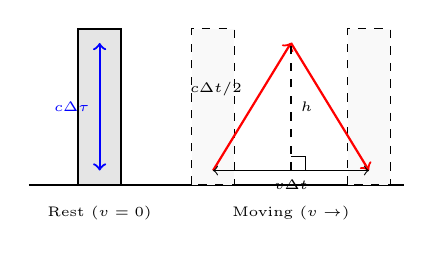
\begin{tikzpicture}[scale=0.9]
                % Ground Line
                \draw[thick] (-0.5, 0) -- (4.8, 0);
                
                % Case A: Rest
                \node at (0.5, -0.4) {\tiny Rest ($v=0$)};
                \draw[thick, fill=gray!20] (0.2, 0) rectangle (0.8, 2.2);
                \draw[<->, blue, thick] (0.5, 0.2) -- (0.5, 2.0) node[midway, left]{\tiny $c\Delta \tau$};
                
                % Case B: Moving
                \node at (3.2, -0.4) {\tiny Moving ($v \to$)};
                % Ghost boxes
                \draw[dashed, fill=gray!5] (1.8, 0) rectangle (2.4, 2.2);
                \draw[dashed, fill=gray!5] (4.0, 0) rectangle (4.6, 2.2);
                
                % Triangle Path
                \draw[->, red, thick] (2.1, 0.2) -- (3.2, 2.0) node[midway, above left, black]{\tiny $c\Delta t/2$};
                \draw[->, red, thick] (3.2, 2.0) -- (4.3, 0.2);
                
                % Height h
                \draw[dashed] (3.2, 0.2) -- (3.2, 2.0) node[midway, right]{\tiny $h$};
                
                % Base v*t
                \draw[<->] (2.1, 0.2) -- (4.3, 0.2) node[midway, below]{\tiny $v\Delta t$};
                
                % Right Angle Symbol
                \draw (3.2, 0.4) -- (3.4, 0.4) -- (3.4, 0.2);
            \end{tikzpicture}
    \end{columns}
\end{frame}

\begin{frame}[shrink=5]{效应判别法 I:时间}
    \begin{columns}[T]
        \column{0.48\textwidth}
            \footnotesize
            \begin{block}{1. 本征时间 (Proper Time) $\Delta \tau$}
                \textbf{定义}:在\textbf{同一地点}发生的两个事件的时间间隔。
                \begin{itemize}
                    \item \textbf{判据}:只需要\textbf{一只钟}就能测出的时间。
                    \item \textit{例子}:飞船上的人看自己的手表;粒子自身的衰变寿命。
                \end{itemize}
            \end{block}

            \begin{block}{2. 测量时间 (Dilated Time) $\Delta t$}
                \textbf{定义}:在\textbf{不同地点}发生的两个事件的时间间隔。
                \begin{itemize}
                    \item \textbf{判据}:需要\textbf{两只}异地同步的钟才能测出(一只在起点,一只在终点)。
                    \item \textit{例子}:地面人看飞船飞过头顶和地平线。
                \end{itemize}
            \end{block}

        \column{0.48\textwidth}
            \small
            \begin{alertblock}{Survival Algorithm: 数钟法}
                拿到题目,不要管谁动谁静,直接数钟:
                \begin{enumerate}
                    \item \textbf{谁在用一只钟测?} $\to$ 他测的是 $\Delta \tau$(数值小)。
                    \item \textbf{谁在用两只钟测?} $\to$ 他测的是 $\Delta t$(数值大)。
                    \item \textbf{公式}:$\Delta t = \gamma \Delta \tau$。
                \end{enumerate}
            \end{alertblock}

            \vspace{0.5em}
            \centering
            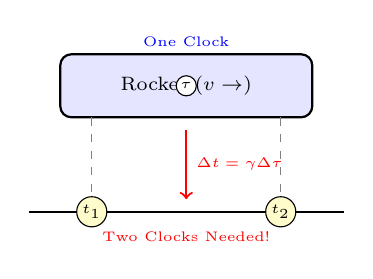
\begin{tikzpicture}[scale=0.8]
                % Moving Frame (Rocket) - One Clock
                \draw[thick, fill=blue!10, rounded corners] (0, 1.5) rectangle (4, 2.5);
                \node at (2, 2.0) {\scriptsize Rocket ($v \to$)};
                \node[draw, circle, fill=white, inner sep=1pt] at (2, 2.0) {\tiny $\tau$};
                \node[blue] at (2, 2.7) {\tiny One Clock};

                % Rest Frame (Ground) - Two Clocks
                \draw[thick] (-0.5, 0) -- (4.5, 0);
                
                % Event 1
                \draw[dashed, gray] (0.5, 1.5) -- (0.5, 0);
                \node[draw, circle, fill=yellow!20, inner sep=1pt] at (0.5, 0) {\tiny $t_1$};
                
                % Event 2
                \draw[dashed, gray] (3.5, 1.5) -- (3.5, 0);
                \node[draw, circle, fill=yellow!20, inner sep=1pt] at (3.5, 0) {\tiny $t_2$};
                
                \node[red] at (2, -0.4) {\tiny Two Clocks Needed!};
                
                % Relationship
                \draw[->, thick, red] (2, 1.3) -- (2, 0.2) node[midway, right]{\tiny $\Delta t = \gamma \Delta \tau$};
            \end{tikzpicture}
            
            \vspace{0.2em}
            \scriptsize{\textbf{记忆}:因为要校准两只钟很麻烦,所以测出来的结果总是“夸大”的 ($\Delta t > \Delta \tau$)。}
    \end{columns}
\end{frame}

\begin{frame}[shrink=8]{时空效应 II:长度收缩}
    \begin{columns}[T]
        \column{0.48\textwidth}
            \footnotesize
            \begin{block}{1. 物理推导 (利用钟慢效应)}
                如何测量一根飞过的尺子长度 $L$?
                \begin{itemize}
                    \item \textbf{实验室系 (Lab)}:设置一个探测器,记录尺子通过的时间 $\Delta t$。
                    $$ L = v \Delta t $$
                    \item \textbf{尺子系 (Rest)}:尺子看探测器飞过,记录时间 $\Delta \tau$ (探测器是单钟)。
                    $$ L_0 = v \Delta t' $$
                    \item \textbf{关联}:由于 $\Delta t'$ 是两地时间 (Lab系的 $\Delta t$),$\Delta t$ 是本征时间 (尺子系的 $\Delta \tau$)... \alert{Wait! 反了!}
                \end{itemize}
                \textbf{正确逻辑}:探测器是“单钟”($\Delta \tau$),尺子上的两端是“双钟”($\Delta t_{dilated}$)。
                $$ L = v \Delta \tau, \quad L_0 = v (\gamma \Delta \tau) \implies L = L_0 / \gamma $$
            \end{block}

        \column{0.48\textwidth}
            \small
            \begin{alertblock}{结论:动尺变短}
                \begin{equation}
                    L = L_0 \sqrt{1 - v^2/c^2} \le L_0
                \end{equation}
                \textbf{关键限制}:收缩仅发生在\textbf{运动方向}上!
                \begin{itemize}
                    \item 纵向:$L_{\parallel} = L_{0} / \gamma$
                    \item 横向:$L_{\perp} = L_{0}$ (不变)
                \end{itemize}
            \end{alertblock}

            \vspace{0.8em}
            \centering
            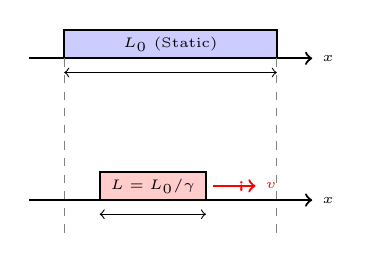
\begin{tikzpicture}[scale=0.9]
                % Static Ruler
                \draw[thick, ->] (0, 2) -- (4, 2) node[right]{\tiny $x$};
                \draw[fill=blue!20, thick] (0.5, 2.0) rectangle (3.5, 2.4);
                \node at (2.0, 2.2) {\tiny $L_0$ (Static)};
                \draw[<->] (0.5, 1.8) -- (3.5, 1.8);
                
                % Moving Ruler
                \draw[thick, ->] (0, 0) -- (4, 0) node[right]{\tiny $x$};
                \draw[fill=red!20, thick] (1.0, 0) rectangle (2.5, 0.4);
                \node at (1.75, 0.2) {\tiny $L = L_0/\gamma$};
                \draw[->, thick, red] (2.6, 0.2) -- (3.2, 0.2) node[right]{\tiny $v$};
                \draw[<->] (1.0, -0.2) -- (2.5, -0.2);
                
                % Vertical Comparison
                \draw[dashed, gray] (0.5, 2.0) -- (0.5, -0.5);
                \draw[dashed, gray] (3.5, 2.0) -- (3.5, -0.5);
                
                \node[red] at (3.0, 0.2) {\textbf{\tiny <}};
            \end{tikzpicture}
            
            \vspace{0.2em}
            \scriptsize{如果原本是球体,运动起来会变成“扁平的饼”。}
    \end{columns}
\end{frame}

\begin{frame}[shrink=5]{效应判别法 II:长度}
    \begin{columns}[T]
        \column{0.40\textwidth} % 左栏变窄,迫使文字换行利用垂直空间
            \footnotesize
            \begin{block}{1. 原长 (Proper Length) $l_0$}
                \textbf{定义}:物体在\textbf{对其静止}的参考系中的长度。
                \begin{itemize}
                    \item \textbf{判据}:测量者与物体无相对运动。
                    \item \textit{性质}:几何真值,数值最大。
                \end{itemize}
            \end{block}

            \begin{block}{2. 测量长度 $l$}
                \textbf{定义}:物体在\textbf{对其运动}的参考系中的长度。
                \begin{itemize}
                    \item \textbf{判据}:物体飞过测量者。
                    \item \textbf{方法}:必须\textbf{同时}测定两端坐标。
                \end{itemize}
            \end{block}

        \column{0.58\textwidth} % 右栏变宽,缓解拥挤
            \small
            \begin{alertblock}{Survival Algorithm: 维度分离法}
                建立坐标系,将长度分解处理:
                \begin{enumerate}
                    \item \textbf{平行分量 ($x \parallel v$)}:
                    $$ l_{\parallel} = l_{0,\parallel} / \gamma \quad (\text{变短}) $$
                    \item \textbf{垂直分量 ($y \perp v$)}:
                    $$ l_{\perp} = l_{0,\perp} \quad (\alert{\textbf{不变!}}) $$
                \end{enumerate}
            \end{alertblock}

            \vspace{0.2em} % 减少间距
            \centering
            % 优化后的紧凑布局
            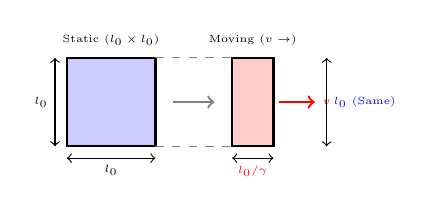
\begin{tikzpicture}[scale=0.75, transform shape]
                % Static Square (Left)
                \draw[thick, fill=blue!20] (0, 0) rectangle (1.5, 1.5);
                \node at (0.75, 1.8) {\tiny Static ($l_0 \times l_0$)};
                \draw[<->] (-0.2, 0) -- (-0.2, 1.5) node[midway, left]{\tiny $l_0$};
                \draw[<->] (0, -0.2) -- (1.5, -0.2) node[midway, below]{\tiny $l_0$};
                
                % Arrow
                \draw[->, thick, gray] (1.8, 0.75) -- (2.5, 0.75);

                % Moving Rectangle (Right)
                \draw[thick, fill=red!20] (2.8, 0) rectangle (3.5, 1.5); % Width halved
                \node at (3.15, 1.8) {\tiny Moving ($v \to$)};
                \draw[->, thick, red] (3.6, 0.75) -- (4.2, 0.75) node[right]{\tiny $v$};
                
                % Dimensions
                \draw[<->] (2.8, -0.2) -- (3.5, -0.2) node[midway, below, red]{\tiny $l_0/\gamma$};
                \draw[<->] (4.4, 0) -- (4.4, 1.5) node[midway, right, blue]{\tiny $l_0$ (Same)};
                
                % Comparison lines
                \draw[dashed, gray] (1.5, 1.5) -- (2.8, 1.5);
                \draw[dashed, gray] (1.5, 0) -- (2.8, 0);
            \end{tikzpicture}
            
            \vspace{0.1em}
            \scriptsize{推论:球体 $\xrightarrow{v}$ 椭球 (垂直方向直径不变)。}
    \end{columns}
\end{frame}

\subsection{洛伦兹变换与运动学}

\begin{frame}[shrink=15]{坐标变换的“算法化”流程}
    \begin{columns}[T]
        \column{0.48\textwidth}
            \footnotesize
                设 $S'$ 相对 $S$ 以速度 $v$ 沿 $+x$ 轴运动。
                \begin{itemize}
                    \item \textbf{去撇 (To $S'$)}: 已知地面,求飞船。
                    \begin{align*}
                        x' &= \gamma(x - vt) \\
                        t' &= \gamma(t - v x/c^2)
                    \end{align*}
                    \item \textbf{回正 (To $S$)}: 已知飞船,求地面。
                    \begin{align*}
                        x &= \gamma(x' + vt') \\
                        t &= \gamma(t' + v x'/c^2)
                    \end{align*}
                \end{itemize}
                \textit{注:$y,z$ 坐标不变。}

            % 将原本在右侧的陷阱移到左侧,填补空白
            \begin{exampleblock}{致命陷阱:$v$ 的正负号}
                如果飞船向\textbf{左}($-x$ 方向)飞,公式里的 $v$ 必须代入\textbf{负值}!
                \begin{itemize}
                    \item 此时“去撇”变加号 $(x+vt)$,“回正”变减号。
                \end{itemize}
            \end{exampleblock}

        \column{0.48\textwidth}
            \footnotesize % 右栏也改用 footnotesize 以防万一
            \begin{alertblock}{Decision Matrix: 坐标变换四步走}
                \begin{enumerate}
                    \item \textbf{建系 (Define)}:
                    \begin{itemize}
                        \item $S$ 系:通常设为地面/实验室。
                        \item $S'$ 系:通常设为飞船/滑块。
                        \item 明确 $v$ 的方向。
                    \end{itemize}
                    
                    \item \textbf{对点 (Map)}:
                    \textbf{绝对不要}直接带入长度 $L$!
                    \\ 必须将物理事件转化为坐标点:
                    \begin{itemize}
                        \item 事件1: $(x_1, t_1)$
                        \item 事件2: $(x_2, t_2)$
                    \end{itemize}

                    \item \textbf{转换 (Transform)}:
                    \begin{itemize}
                        \item 求 $x', t'$ $\to$ 用去撇公式。
                        \item 求 $x, t$ $\to$ 用回正公式。
                        \item 求间隔 $\to$ 直接用 $\Delta$ 形式。
                    \end{itemize}

                    \item \textbf{计算 (Calculate)}:
                    小心 $\gamma$ 因子的计算,保留 $c$ 直到最后约掉。
                \end{enumerate}
            \end{alertblock}
    \end{columns}
\end{frame}

\begin{frame}[shrink=5]{速度合成定理}
    \begin{columns}[T]
        \column{0.48\textwidth}
            \footnotesize
                设物体在 $S'$ 系速度为 $\vec{u}'(u'_x, u'_y)$,求在 $S$ 系速度 $\vec{u}$。
                \begin{itemize}
                    \item \textbf{纵向分量 ($x \parallel v$)}:
                    \begin{equation}
                        u_x = \frac{u'_x + v}{1 + \frac{v u'_x}{c^2}}
                    \end{equation}
                    \item \textbf{横向分量 ($y \perp v$)}:
                    \begin{equation}
                        u_y = \frac{u'_y}{\gamma(1 + \frac{v u'_x}{c^2})}
                    \end{equation}
                \end{itemize}
                \textit{注意:$u_y$ 的分母不仅有修正项,还有 $\gamma$ 因子!}

            \begin{exampleblock}{逆变换技巧}
                已知 $u$ 求 $u'$?$\implies$ 只需将 $v$ 换成 $-v$。
                $$ u'_x = \frac{u_x - v}{1 - \frac{v u_x}{c^2}} $$
            \end{exampleblock}

        \column{0.48\textwidth}
            \footnotesize
            \begin{alertblock}{Survival Tip: 分式记忆法}
                \begin{itemize}
                    \item \textbf{分子}:经典伽利略变换 ($u'_x + v$)。
                    \item \textbf{分母}:相对论修正因子 $(1 + \beta_v \beta_{u'})$。
                \end{itemize}
            \end{alertblock}

            \vspace{0.3em}
            \centering
            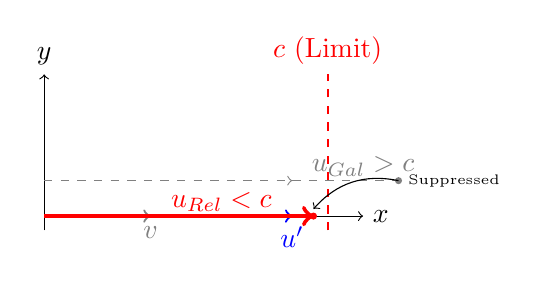
\begin{tikzpicture}[scale=0.9]
                % Axes
                \draw[->] (0,0) -- (4.5,0) node[right] {$x$};
                \draw[->] (0,-0.2) -- (0,2) node[above] {$y$};
                
                % C barrier
                \draw[dashed, red, thick] (4, -0.2) -- (4, 2);
                \node[red, anchor=south] at (4, 2) {$c$ (Limit)};
                
                % Vectors
                \draw[->, thick, gray] (0,0) -- (1.5,0) node[below]{$v$};
                \draw[->, thick, blue] (1.5,0) -- (3.5,0) node[below]{$u'$};
                
                % Classical Sum
                \draw[->, dashed, gray] (0,0.5) -- (3.5, 0.5); 
                \draw[dashed, gray] (3.5, 0.5) -- (5.0, 0.5);
                \node[gray] at (4.5, 0.7) {$u_{Gal} > c$};
                \fill[gray] (5.0, 0.5) circle (0.05);
                
                % Relativistic Sum
                \draw[->, red, ultra thick] (0,0) -- (3.8, 0);
                \node[red] at (2.5, 0.2) {$u_{Rel} < c$};
                \fill[red] (3.8, 0) circle (0.05);
                
                % Logic
                \draw[->, bend right] (5.0, 0.5) to (3.8, 0.1);
                \node[right, font=\tiny] at (5.0, 0.5) {Suppressed};
            \end{tikzpicture}
            
            \vspace{0.2em}
            \scriptsize{\textbf{极限检查}:若 $u'=c$,则无论 $v$ 多大,\newline $\frac{c+v}{1+vc/c^2} = \frac{c(c+v)}{c+v} = c$。}
    \end{columns}
\end{frame}

\begin{frame}[shrink=10]{速度变换进阶:角度与光行差}
    \begin{columns}[T]
        \column{0.48\textwidth}
            \footnotesize
            \begin{block}{1. 角度变换公式}
                设粒子在 $S'$ 系中速度方向与 $x'$ 轴夹角为 $\theta'$。
                在 $S$ 系中,利用 $u_y/u_x$:
                \begin{equation}
                    \tan \theta = \frac{u_y}{u_x} = \frac{u'_y \sqrt{1-\beta^2}}{u'_x + v} = \frac{\sin \theta' \sqrt{1-\beta^2}}{\cos \theta' + \beta_{rel}}
                \end{equation}
                \textit{注:此处 $\beta_{rel} = v/u'$。若为光子,则 $\beta_{rel} = v/c = \beta$。}
            \end{block}

            \begin{block}{2. 光行差公式 (对于光子 $u'=c$)}
                更常用的余弦形式:
                \begin{equation}
                    \cos \theta = \frac{\cos \theta' + \beta}{1 + \beta \cos \theta'}
                \end{equation}
                \textbf{极限}:当 $\beta \to 1$ 时,无论 $\theta'$ 是多少(只要不是 $\pi$),$\cos \theta \to 1$,即 $\theta \to 0$。
            \end{block}

        \column{0.48\textwidth}
            \small
            \begin{alertblock}{Survival Intuition: 雨中奔跑}
                为什么星光会向前聚集?
                \begin{itemize}
                    \item \textbf{经典类比}:雨垂直下落,你在雨中奔跑,感觉雨是从“前上方”打来的。
                    \item \textbf{相对论修正}:不仅方向偏转,光强也会因为多普勒效应增强(变蓝)。
                \end{itemize}
            \end{alertblock}

            \vspace{0.5em}
            \centering
            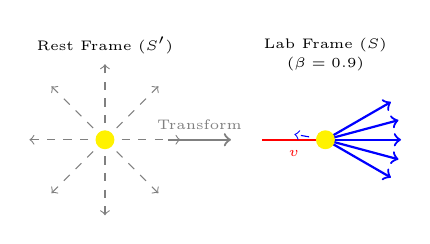
\begin{tikzpicture}[scale=0.8]
                % Isotropic Source (S')
                \node at (0, 1.5) {\tiny Rest Frame ($S'$)};
                \foreach \a in {0, 45, ..., 315}
                    \draw[->, gray, dashed] (0,0) -- (\a:1.2);
                \fill[yellow] (0,0) circle (0.15);

                % Beamed Source (S)
                \begin{scope}[xshift=3.5cm]
                    \node at (0, 1.5) {\tiny Lab Frame ($S$)};
                    \node at (0, 1.2) {\tiny ($\beta=0.9$)};
                    \draw[->, thick, red] (-1,0) -- (0,0) node[midway, below]{\tiny $v$};
                    
                    % Beamed rays
                    \draw[->, blue, thick] (0,0) -- (0:1.2);    % 0 -> 0
                    \draw[->, blue, thick] (0,0) -- (15:1.2);   % 45 -> small
                    \draw[->, blue, thick] (0,0) -- (-15:1.2);  % -45 -> small
                    \draw[->, blue, thick] (0,0) -- (30:1.2);   % 90 -> forward
                    \draw[->, blue, thick] (0,0) -- (-30:1.2);  % -90 -> forward
                    
                    % Backward ray (hard to turn)
                    \draw[->, blue, dashed] (0,0) -- (170:0.5); 
                    
                    \fill[yellow] (0,0) circle (0.15);
                \end{scope}
                
                % Arrow
                \draw[->, thick, gray] (1.0, 0) -- (2.0, 0) node[midway, above]{\tiny Transform};
            \end{tikzpicture}
            
            \vspace{0.2em}
            \scriptsize{\textbf{探照灯效应 (Headlight Effect)}:高速飞船看到的视场会急剧收缩成前方的明亮光锥。}
    \end{columns}
\end{frame}

\begin{frame}[shrink=5]{相对论多普勒效应}
    \begin{columns}[T]
        \column{0.48\textwidth}
            \footnotesize
            \textbf{1. 纵向效应 (Longitudinal):}当光源与观测者沿连线运动时($\vec{v} \parallel \vec{r}$):
                \begin{equation}
                    \nu = \nu_0 \sqrt{\frac{1+\beta}{1-\beta}} \quad (\text{接近, 蓝移})
                \end{equation}
                \begin{equation}
                    \nu = \nu_0 \sqrt{\frac{1-\beta}{1+\beta}} \quad (\text{远离, 红移})
                \end{equation}
                \textit{物理来源:经典多普勒 + 时间延缓。}

            \textbf{2. 横向效应 (Transverse):}当运动方向与视线垂直时($\theta=90^\circ$, 最近点):
                \begin{equation}
                    \nu = \nu_0 \sqrt{1-\beta^2} = \frac{\nu_0}{\gamma} \quad (\text{红移})
                \end{equation}
                \alert{\textbf{纯相对论效应}}:经典理论预测此时无频移,但相对论中因为“动钟变慢”,光源频率显得低了。

        \column{0.48\textwidth}
            \small
            \begin{alertblock}{Survival Comparison: 介质去哪了?}
                经典声波多普勒公式繁琐是因为有“风”(介质)。
                相对论光波多普勒公式简洁是因为**没有以太**。
                \begin{itemize}
                    \item 只与相对速度 $v$ 有关。
                    \item 完美对称:谁看谁都一样。
                \end{itemize}
            \end{alertblock}

            \vspace{0.8em}
            \centering
            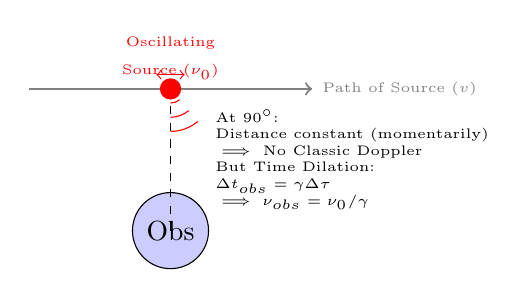
\begin{tikzpicture}[scale=0.9]
                % Observer
                \node[draw, circle, fill=blue!20] (O) at (0,0) {Obs};
                
                % Source Path
                \draw[->, thick, gray] (-2, 2) -- (2, 2) node[right]{\tiny Path of Source ($v$)};
                \draw[dashed] (0,0) -- (0,2);
                
                % Transverse Point
                \fill[red] (0,2) circle (0.15) node[above]{\tiny Source ($\nu_0$)};
                \draw[<->, red] (0.2, 2.2) -- (-0.2, 2.2) node[midway, above=0.2cm]{\tiny Oscillating};
                
                % Wavefronts
                \draw[red, thin] (0,1.8) arc (-90:-50:0.2);
                \draw[red, thin] (0,1.6) arc (-90:-50:0.4);
                \draw[red, thin] (0,1.4) arc (-90:-50:0.6);
                
                % Time Dilation Logic
                \node[right, align=left, font=\tiny] at (0.5, 1.0) {
                    At $90^\circ$:\\
                    Distance constant (momentarily)\\
                    $\implies$ No Classic Doppler\\
                    But Time Dilation:\\
                    $\Delta t_{obs} = \gamma \Delta \tau$\\
                    $\implies \nu_{obs} = \nu_0 / \gamma$
                };
            \end{tikzpicture}
    \end{columns}
\end{frame}

\subsection{相对论动力学基础}

\begin{frame}[shrink=8]{动力学重构 I:质量与动量}
    \begin{columns}[T]
        \column{0.48\textwidth}
            \footnotesize
            \begin{block}{1. 质量的相对性}
                为了保持动量守恒定律在所有惯性系中形式不变,质量必须是速度的函数:
                \begin{equation}
                    m(v) = \gamma m_0 = \frac{m_0}{\sqrt{1 - v^2/c^2}}
                \end{equation}
                \begin{itemize}
                    \item $m_0$:\textbf{静质量} (Rest Mass),内禀属性。
                    \item $m$:\textbf{动质量} (Relativistic Mass),随 $v$ 增大。
                \end{itemize}
            \end{block}

            \begin{block}{2. 动量的新定义}
                \begin{equation}
                    \vec{p} = m \vec{v} = \gamma m_0 \vec{v}
                \end{equation}
                \textbf{推论}:当 $v \to c$ 时,$\gamma \to \infty$,动量 $p \to \infty$。
            \end{block}

        \column{0.48\textwidth}
            \small
            \begin{alertblock}{Survival Intuition: 为什么超不过 $c$?}
                \textbf{经典直觉}:只要一直推,速度就能一直加。
                \textbf{相对论修正}:推得越快,物体变得越“重”(惯性越大)。
                \begin{itemize}
                    \item 当 $v \to c$,惯性 $m \to \infty$。
                    \item 想要继续加速,需要无穷大的力。
                \end{itemize}
            \end{alertblock}

            \vspace{0.8em}
            \centering
            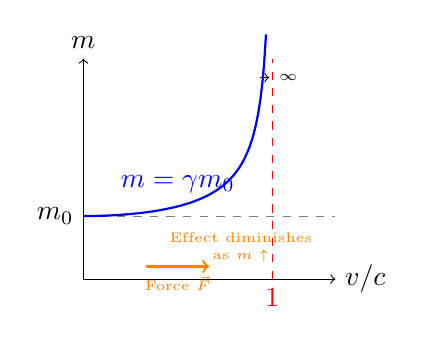
\begin{tikzpicture}[scale=0.8]
                % Axes
                \draw[->] (0,0) -- (4,0) node[right] {$v/c$};
                \draw[->] (0,0) -- (0,3.5) node[above] {$m$};
                
                % Limit Line
                \draw[dashed, red] (3,0) -- (3,3.5);
                \node[red, below] at (3,0) {1};
                
                % m0 Level
                \draw[dashed, gray] (0,1) -- (4,1);
                \node[left] at (0,1) {$m_0$};
                
                % Curve
                \draw[thick, blue, domain=0:2.9, samples=100] plot (\x, {1/sqrt(1-(\x/3)^2)});
                
                % Annotation
                \node[blue] at (1.5, 1.5) {$m = \gamma m_0$};
                \draw[->] (2.8, 3.2) -- (2.95, 3.2) node[right, font=\tiny]{$\infty$};
                
                % Force Arrow
                \draw[->, orange, thick] (1, 0.2) -- (2, 0.2) node[midway, below]{\tiny Force $\vec{F}$};
                \node[orange, font=\tiny, align=center] at (2.5, 0.5) {Effect diminishes\\ as $m \uparrow$};
            \end{tikzpicture}
            
            \vspace{0.2em}
            \scriptsize{注:在现代粒子物理中,通常只说“质量”指 $m_0$,不再强调动质量 $m$。}
    \end{columns}
\end{frame}

\begin{frame}[shrink=10]{动力学重构 II:动能}
    \begin{columns}[T]
        \column{0.48\textwidth}
            \footnotesize
            \begin{block}{1. 动能的严格定义}
                动能 = 外力对静止物体做的功 = 总能 - 静能。
                \begin{equation}
                    E_k = \int_0^x F dx = E - E_0 = (\gamma - 1)m_0 c^2
                \end{equation}
                \textbf{推论}:
                \begin{itemize}
                    \item 当 $v=0, \gamma=1 \implies E_k=0$。
                    \item 当 $v \to c, \gamma \to \infty \implies E_k \to \infty$。
                \end{itemize}
            \end{block}

            \begin{block}{2. 低速极限 (Low Speed Limit)}
                当 $v \ll c$ ($\beta \ll 1$) 时,利用泰勒展开 $\gamma \approx 1 + \frac{1}{2}\beta^2$:
                \begin{align*}
                    E_k &\approx (1 + \frac{1}{2}\frac{v^2}{c^2} - 1) m_0 c^2 \\
                        &= \frac{1}{2} m_0 v^2 \quad (\text{牛顿力学})
                \end{align*}
            \end{block}

        \column{0.48\textwidth}
            \footnotesize
            \begin{alertblock}{Survival Warning: 绝对禁区}
                \alert{\textbf{严禁}} 使用 $E_k = \frac{1}{2}m v^2$ 或 $E_k = \frac{1}{2}m(v) v^2$!
                \begin{itemize}
                    \item 经典公式只在 $v \lesssim 0.1c$ 时近似成立。
                    \item 在高能物理中,动能通常远大于静能 ($E_k \gg m_0 c^2$),此时 $E \approx E_k \approx pc$。
                \end{itemize}
            \end{alertblock}

            \vspace{0.3em}
            \centering
            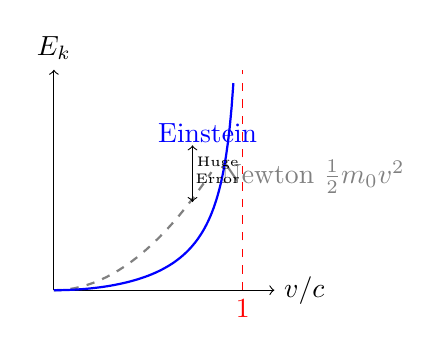
\begin{tikzpicture}[scale=0.8]
                % Axes
                \draw[->] (0,0) -- (3.5,0) node[right] {$v/c$};
                \draw[->] (0,0) -- (0,3.5) node[above] {$E_k$};
                
                % Limit Line
                \draw[dashed, red] (3,0) -- (3,3.5);
                \node[red, below] at (3,0) {1};
                
                % Classical Parabola 0.5 * x^2 (scaled)
                \draw[dashed, gray, thick] plot[domain=0:2.5] (\x, {0.3*\x*\x});
                \node[gray, right] at (2.5, 1.8) {Newton $\frac{1}{2}m_0 v^2$};
                
                % Relativistic Curve (1/sqrt(1-x^2) - 1)
                \draw[thick, blue, samples=100, domain=0:2.85] plot (\x, {1.5*(1/sqrt(1-(\x/3)^2) - 1)});
                \node[blue, right] at (1.5, 2.5) {Einstein};
                
                % Comparison Arrow
                \draw[<->] (2.2, 1.4) -- (2.2, 2.3);
                \node[font=\tiny, align=center] at (2.6, 1.9) {Huge\\Error};
            \end{tikzpicture}
            
            \vspace{0.2em}
            \scriptsize{随着速度接近 $c$,注入的能量不再增加速度,而是增加质量(惯性)。}
    \end{columns}
\end{frame}

\begin{frame}[shrink=15]{几何化思维:能量-动量三角形}
    \begin{columns}[T]
        \column{0.45\textwidth}
            \footnotesize
            \begin{block}{1. 勾股定理关系}
                由 $E = \gamma m_0 c^2$ 和 $p = \gamma m_0 v$,消去 $v$ 可得:
                \begin{equation}
                    E^2 = (pc)^2 + (m_0 c^2)^2
                \end{equation}
                这构成了一个直角三角形:
                \begin{itemize}
                    \item \textbf{斜边}:总能量 $E$
                    \item \textbf{直角边}:动量项 $pc$,静能 $m_0 c^2$
                \end{itemize}
            \end{block}

            \begin{block}{2. 角度的物理意义}
                在这个三角形中,角度直接对应速度:
                \begin{align}
                    \sin \theta &= \frac{pc}{E} = \frac{\gamma m_0 v \cdot c}{\gamma m_0 c^2} = \frac{v}{c} = \beta \\
                    \cos \theta &= \frac{m_0 c^2}{E} = \frac{1}{\gamma}
                \end{align}
                \textit{推论:能量越高,$\theta \to 90^\circ$,速度越接近 $c$。}
            \end{block}

        \column{0.53\textwidth}
            \centering
            \begin{tikzpicture}[scale=1.5]
                % Axes
                \draw[->] (-0.2,0) -- (2.2,0) node[right] {$pc$};
                \draw[->] (0,-0.2) -- (0,1.8) node[above] {$E$}; % Note: E is usually hypotenuse, but plotting on E-pc plane? 
                % Actually better to draw the triangle explicitly
                
                % Triangle
                \draw[ultra thick, blue] (0,0) -- (1.8,0) node[midway, below] {$pc$};
                \draw[ultra thick, red] (0,0) -- (0,1.2) node[midway, left] {$m_0 c^2$};
                \draw[ultra thick, green!60!black] (0,1.2) -- (1.8,0) node[midway, above right] {$E$};
                
                % Angle
                \draw (1.5,0) arc (180:146:0.3);
                \node at (1.35, 0.15) {\tiny $\theta$};
                
                % Formula Box
                \node[right, align=left, fill=yellow!10, rounded corners] at (0.2, 1.8) {
                    \textbf{Survival Skill:}\\
                    $\beta = \frac{\text{对边}}{\text{斜边}}$\\
                    $E_k = \text{斜边} - \text{竖直边}$
                };
            \end{tikzpicture}
            
            \vspace{0.5em}
            \small
            \begin{alertblock}{极高能极限 (Ultra-relativistic)}
                当 $E \gg m_0 c^2$ 时 (如 LHC 质子):
                \begin{itemize}
                    \item 直角边 $m_0 c^2$ 忽略不计。
                    \item 三角形退化为直线 $\implies E \approx pc$。
                    \item $\beta \approx 1$ (速度 $v \approx c$)。
                \end{itemize}
            \end{alertblock}
    \end{columns}
\end{frame}

\begin{frame}[shrink=15]{动力学重构 III:力与加速度}
    \begin{columns}[T]
        \column{0.48\textwidth}
            \footnotesize
            \begin{block}{1. 牛顿第二定律的修正}
                在相对论中,力定义为\textbf{动量的变化率},而非质量乘以加速度:
                \begin{equation}
                    \vec{F} = \frac{d\vec{p}}{dt} = \frac{d}{dt}(\gamma m_0 \vec{v})
                \end{equation}
                展开后发现 $\vec{F}$ 与 $\vec{a}$ \textbf{不一定同向}!
            \end{block}

            \begin{block}{2. 纵向与横向质量 (已弃用的概念)}
                \begin{itemize}
                    \item \textbf{纵向 ($F \parallel v$)}:加速极其困难。
                    $$ F = \gamma^3 m_0 a \implies m_L = \gamma^3 m_0 $$
                    \item \textbf{横向 ($F \perp v$)}:转弯相对容易。
                    $$ F = \gamma m_0 a \implies m_T = \gamma m_0 $$
                \end{itemize}
                \textit{注:由于质量居然随方向变化,现代物理已弃用此说法,统称 $m_0$ 为质量。}
            \end{block}

        \column{0.48\textwidth}
            \small
            \begin{alertblock}{Survival Tip: 为什么要用能量法?}
                因为力学方程太丑了!
                \begin{itemize}
                    \item 在 $S$ 系算力,既有 $\gamma$ 又有 $\gamma^3$,积分极其痛苦。
                    \item \textbf{最优解}:使用功能原理 $W = \Delta E_k$ 或动量守恒。
                \end{itemize}
            \end{alertblock}

            \vspace{0.5em}
            \centering
            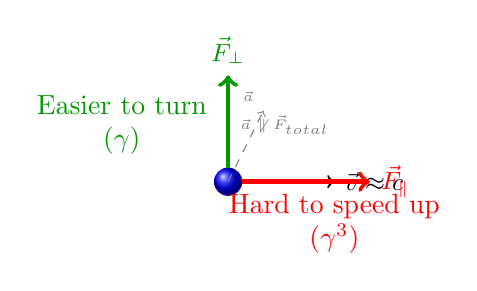
\begin{tikzpicture}[scale=0.9]
                % Particle
                \draw[->, thick] (0,0) -- (1.5,0) node[right]{\small $\vec{v} \approx c$};
                \shade[ball color=blue] (0,0) circle (0.2);
                
                % Longitudinal Force
                \draw[->, red, ultra thick] (0.2, 0) -- (2.0, 0) node[right]{\small $\vec{F}_{\parallel}$};
                \node[red, align=center] at (1.5, -0.6) {Hard to speed up\\($\gamma^3$)};
                
                % Transverse Force
                \draw[->, green!60!black, ultra thick] (0, 0.2) -- (0, 1.5) node[above]{\small $\vec{F}_{\perp}$};
                \node[green!60!black, align=center] at (-1.5, 0.8) {Easier to turn\\($\gamma$)};
                
                % Acceleration Vector (Resultant)
                \draw[dashed, gray, ->] (0,0) -- (0.5, 1.0) node[above left]{\tiny $\vec{a}$};
                \node[gray, font=\tiny] at (0.8, 0.8) {$\vec{a} \not\parallel \vec{F}_{total}$};
            \end{tikzpicture}
            
            \vspace{0.2em}
            \scriptsize{这就解释了为什么回旋加速器 (Cyclotron) 无法加速高能电子——因为 $m$ 变了,回旋周期 $T$ 不再恒定。}
    \end{columns}
\end{frame}

\begin{frame}[shrink=15]{零静质量粒子:光子 (Photons)}
    \begin{columns}[T]
        \column{0.48\textwidth}
            \footnotesize
            \begin{block}{1. 状态方程}
                光子 (Photon) 的定义特征是静质量为零:
                $$ m_0 \equiv 0 $$
                代入能量-动量关系 $E^2 - p^2 c^2 = m_0^2 c^4$:
                \begin{equation}
                    E = pc \implies p = \frac{E}{c}
                \end{equation}
                \textbf{速度}:$v = \frac{pc^2}{E} = c$ (恒定光速)。
            \end{block}

            \begin{block}{2. 与量子力学的接口}
                普朗克-爱因斯坦关系 (Planck-Einstein):
                \begin{equation}
                    E = h\nu = \hbar \omega
                \end{equation}
                \begin{equation}
                    \vec{p} = \hbar \vec{k} \quad (|\vec{k}| = 2\pi/\lambda)
                \end{equation}
                \textit{光子虽无质量,但有动量!这是光压的来源。}
            \end{block}

        \column{0.48\textwidth}
            \small
            \begin{alertblock}{Survival Warning: 光子的禁区}
                \begin{itemize}
                    \item \textbf{禁区 1}:绝对不要对光子使用 $\gamma$ 或 $m_0 \gamma$ 公式(因为 $\gamma \to \infty$)。
                    \item \textbf{禁区 2}:光子没有“静止系”。你不能骑在光子上看世界(时间停止,距离为零)。
                \end{itemize}
            \end{alertblock}

            \vspace{0.5em}
            \centering
            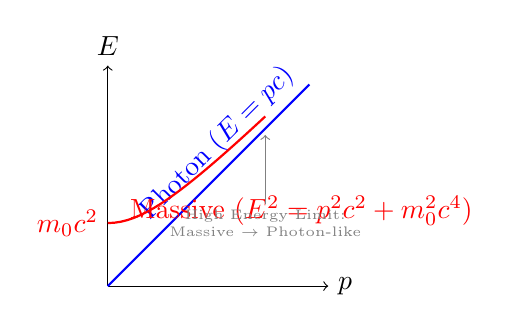
\begin{tikzpicture}[scale=0.8]
                % Axes
                \draw[->] (0,0) -- (3.5,0) node[right] {$p$};
                \draw[->] (0,0) -- (0,3.5) node[above] {$E$};
                
                % Photon Line
                \draw[thick, blue] (0,0) -- (3.2, 3.2);
                \node[blue, rotate=45, anchor=south] at (2.0, 2.0) {Photon ($E=pc$)};
                
                % Massive Particle Curve
                \draw[thick, red, domain=0:2.5] plot (\x, {sqrt(\x*\x + 1)});
                \node[red, anchor=west] at (0.2, 1.2) {Massive ($E^2 = p^2c^2 + m_0^2c^4$)};
                \draw[dashed, red] (0,1) -- (0.1,1);
                \node[left, red] at (0,1) {$m_0 c^2$};
                
                % Asymptote behavior
                \node[gray, font=\tiny, align=center] at (2.5, 1.0) {High Energy Limit:\\Massive $\to$ Photon-like};
                \draw[->, gray] (2.5, 1.3) -- (2.5, 2.4);
            \end{tikzpicture}
            
            \vspace{0.2em}
            \scriptsize{这就解释了为什么极高能电子($E \gg m_e c^2$)的行为非常像光子。}
    \end{columns}
\end{frame}

\subsection{碰撞、衰变与守恒律}

\begin{frame}[shrink=5]{碰撞与衰变的神器:不变质量法}
    \begin{columns}[T]
        \column{0.48\textwidth}
            \footnotesize
            \begin{block}{1. 单粒子不变量}
                我们在几何化思维中已经知道,对于任意粒子:
                $$ E^2 - p^2 c^2 = m_0^2 c^4 = \text{Invariant} $$
                无论你在哪个参考系算,$E$ 和 $p$ 会变,但“斜边平方减直角边平方”永远等于静能平方。
            \end{block}

            \begin{block}{2. 多粒子系统不变量 (Mandelstam $s$)}
                对于孤立系统(如碰撞前后),定义总能量 $E_{tot}$ 和总动量 $\vec{p}_{tot}$。
                \textbf{不变质量} $M$ 定义为:
                \begin{equation}
                    M^2 c^4 = (\sum E_i)^2 - (\sum \vec{p}_i c)^2 \equiv s
                \end{equation}
                \textbf{核心性质}:$s_{\text{Lab}} = s_{\text{COM}}$
                \\ (实验室系的值 = 质心系的值)
            \end{block}

        \column{0.48\textwidth}
            \small
            \begin{alertblock}{Survival Algorithm: 为什么不用守恒律?}
                直接列能量/动量守恒方程组通常会引入速度 $v$ 和 $\gamma$,计算极其繁琐。
                \textbf{不变质量法}的优势:
                \begin{itemize}
                    \item \textbf{绕过速度}:直接处理 $E$ 和 $p$。
                    \item \textbf{系间跳跃}:利用 $s$ 不变,瞬间连接实验室系与质心系。
                \end{itemize}
            \end{alertblock}

            \vspace{0.5em}
            \centering
            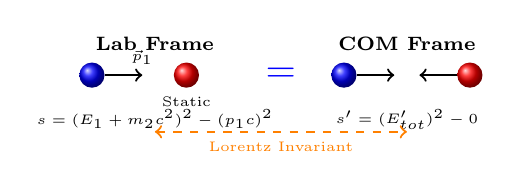
\begin{tikzpicture}[scale=0.8]
                % Lab Frame
                \node at (0, 2.0) {\scriptsize \textbf{Lab Frame}};
                \shade[ball color=blue] (-1.0, 1.5) circle (0.2);
                \draw[->, thick] (-0.8, 1.5) -- (-0.2, 1.5) node[above]{\tiny $\vec{p}_1$};
                \shade[ball color=red] (0.5, 1.5) circle (0.2);
                \node[below] at (0.5, 1.3) {\tiny Static};
                \node at (0, 0.8) {\tiny $s = (E_1+m_2c^2)^2 - (p_1c)^2$};
                
                % Equality
                \node[font=\Large, blue] at (2.0, 1.5) {$=$};
                
                % COM Frame
                \node at (4.0, 2.0) {\scriptsize \textbf{COM Frame}};
                \shade[ball color=blue] (3.0, 1.5) circle (0.2);
                \draw[->, thick] (3.2, 1.5) -- (3.8, 1.5);
                \shade[ball color=red] (5.0, 1.5) circle (0.2);
                \draw[->, thick] (4.8, 1.5) -- (4.2, 1.5);
                \node at (4.0, 0.8) {\tiny $s' = (E'_{tot})^2 - 0$};
                
                % Bridge
                \draw[<->, dashed, thick, orange] (0, 0.6) -- (4.0, 0.6) node[midway, below]{\tiny Lorentz Invariant};
            \end{tikzpicture}
            
            \vspace{0.2em}
            \scriptsize{这是高能物理中计算“阈值能量”的唯一指定方法。}
    \end{columns}
\end{frame}

\begin{frame}[shrink=20]{不变质量法 II:阈值能量计算范式}
    \begin{columns}[T]
        \column{0.48\textwidth}
            \footnotesize
            \begin{block}{1. 阈值的物理定义}
                \textbf{什么是阈值?}
                使核反应 $A + B \to C + D + \dots$ 能够发生的最小入射能量。
                \begin{itemize}
                    \item \textbf{动力学条件}:在\textbf{质心系 (COM)} 中,反应后的所有产物\textbf{相对静止}。
                    \item \textbf{物理本质}:动能全部转化为静质量 (能损最大化)。
                \end{itemize}
            \end{block}

            \begin{alertblock}{2. 标准解题算法}
                利用不变量 $s_{\text{Lab}} = s_{\text{COM}}$:
                \begin{enumerate}
                    \item 写出实验室系总四维动量平方 $s$。
                    \item 写出质心系(阈值态)总四维动量平方 $s'$。
                    \item 令 $s = s'$,解出 $E$。
                \end{enumerate}
            \end{alertblock}

            \vspace{0.2em}
            \centering
            % 将图移到左侧填补空白
            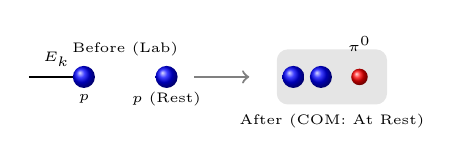
\begin{tikzpicture}[scale=0.7]
                % Before
                \draw[->, thick] (-1, 0) -- (0, 0) node[midway, above]{\tiny $E_k$};
                \shade[ball color=blue] (0, 0) circle (0.2); \node at (0, -0.4) {\tiny $p$};
                \shade[ball color=blue] (1.5, 0) circle (0.2); \node at (1.5, -0.4) {\tiny $p$ (Rest)};
                \node at (0.75, 0.5) {\tiny Before (Lab)};
                
                \draw[->, thick, gray] (2.0, 0) -- (3.0, 0);
                
                % After
                \fill[gray!20, rounded corners] (3.5, -0.5) rectangle (5.5, 0.5);
                \shade[ball color=blue] (3.8, 0) circle (0.2);
                \shade[ball color=blue] (4.3, 0) circle (0.2);
                \shade[ball color=red] (5.0, 0) circle (0.15) node[above=0.2cm]{\tiny $\pi^0$};
                \node at (4.5, -0.8) {\tiny After (COM: At Rest)};
            \end{tikzpicture}

        \column{0.48\textwidth}
            \footnotesize % 右栏也用 footnotesize 防止溢出
            \begin{exampleblock}{Survival Example: $p + p \to p + p + \pi^0$}
                求入射质子(静能 $m$)的最小动能 $E_k$。
                
                \textbf{Step 1: Lab系 (始态)}
                \\ 入射 $(E, p)$,靶 $(mc^2, 0)$。
                \begin{align*}
                    s &= (E + mc^2)^2 - (pc)^2 \\
                      &= E^2 + 2Emc^2 + m^2c^4 - p^2c^2 \\
                      &= \underbrace{(E^2 - p^2c^2)}_{m^2c^4} + 2Emc^2 + m^2c^4 \\
                      &= 2mc^2(E + mc^2)
                \end{align*}
                
                \textbf{Step 2: COM系 (末态)}
                \\ 产物总静能 $M = 2m + m_\pi$。所有粒子相对静止 $\implies$ 动量为0。
                $$ s' = (Mc^2)^2 - 0 = (2m + m_\pi)^2 c^4 $$
                
                \textbf{Step 3: 求解}
                \\ 令 $s=s'$,解出 $E$:
                $$ 2mc^2(E + mc^2) = (2m+m_\pi)^2 c^4 $$
                $$ E_k = E - mc^2 = \frac{(2m+m_\pi)^2 c^2}{2m} - 2mc^2 $$
                \scriptsize{(结果约为 $290\text{MeV}$)}
            \end{exampleblock}
    \end{columns}
\end{frame}

\begin{frame}[shrink=12]{康普顿散射}
    \begin{columns}[T]
        \column{0.48\textwidth}
            \footnotesize
            \begin{block}{1. 物理图像与守恒律}
                入射光子 ($\lambda, E$) 撞击静止电子 ($m_e$),散射后光子变长 ($\lambda', E'$),电子反冲。
                \begin{itemize}
                    \item \textbf{能量守恒}:
                    $$ h\nu + m_e c^2 = h\nu' + E_e $$
                    \item \textbf{动量守恒} (矢量三角形):
                    $$ \vec{p}_\gamma = \vec{p}'_\gamma + \vec{p}_e \implies \vec{p}_e = \vec{p}_\gamma - \vec{p}'_\gamma $$
                \end{itemize}
            \end{block}

            \begin{block}{2. 推导核心技巧 (消去 $\phi$)}
                为了消去电子角度,对动量式平方(余弦定理):
                $$ p_e^2 = p^2 + p'^2 - 2pp' \cos\theta $$
                利用 $p_e^2 c^2 = E_e^2 - m_e^2 c^4$,代入能量关系化简可得公式。
            \end{block}

        \column{0.48\textwidth}
            \small
            \begin{alertblock}{3. 康普顿公式 (The Formula)}
                波长的偏移量 $\Delta \lambda$ 仅与散射角 $\theta$ 有关:
                \begin{equation}
                    \Delta \lambda = \lambda' - \lambda = \lambda_c (1 - \cos \theta)
                \end{equation}
                \textbf{康普顿波长}:$\lambda_c = \frac{h}{m_e c} \approx 0.00243 \text{nm}$
            \end{alertblock}

            \vspace{0.5em}
            \centering
            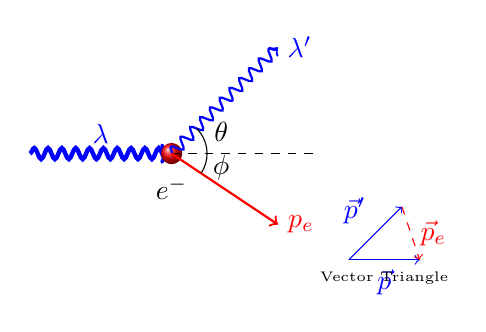
\begin{tikzpicture}[scale=0.9]
                % Incoming Photon
                \draw[->, blue, ultra thick, decorate, decoration={snake, amplitude=2pt, segment length=5pt}] (-2, 0) -- (0, 0);
                \node[blue, above] at (-1, 0) {$\lambda$};
                
                % Target Electron
                \shade[ball color=red] (0, 0) circle (0.15);
                \node[below] at (0, -0.2) {$e^-$};
                
                % Scattered Photon
                \draw[->, blue, thick, decorate, decoration={snake, amplitude=2pt, segment length=5pt}] (0, 0) -- (1.5, 1.5);
                \node[blue, right] at (1.5, 1.5) {$\lambda'$};
                \draw[dashed] (0,0) -- (2,0);
                \draw (0.5,0) arc (0:45:0.5);
                \node at (0.7, 0.3) {$\theta$};
                
                % Recoil Electron
                \draw[->, red, thick] (0, 0) -- (1.5, -1.0) node[right]{$p_e$};
                \draw (0.5,0) arc (0:-33:0.5);
                \node at (0.7, -0.2) {$\phi$};
                
                % Momentum Triangle (Inset)
                \begin{scope}[shift={(2.5, -1.5)}, scale=0.5]
                    \draw[->, blue] (0,0) -- (2,0) node[midway, below]{$\vec{p}$};
                    \draw[->, blue] (0,0) -- (1.5, 1.5) node[midway, above left]{$\vec{p}'$};
                    \draw[->, red, dashed] (1.5, 1.5) -- (2,0) node[midway, right]{$\vec{p}_e$};
                    \node[font=\tiny] at (1.0, -0.5) {Vector Triangle};
                \end{scope}
            \end{tikzpicture}
            
            \vspace{0.2em}
            \scriptsize{\textbf{极限}:$\theta=180^\circ$ (背散射) 时,$\Delta \lambda$ 最大 ($2\lambda_c$),光子损失能量最多。}
    \end{columns}
\end{frame}

\subsection{高阶拓展:四维时空}

\begin{frame}[shrink=10]{进阶视点 I:闵氏时空与度规}
    \begin{columns}[T]
        \column{0.48\textwidth}
            \footnotesize
            \begin{block}{1. 时空间隔 (Interval)}
                洛伦兹变换的本质是保持\textbf{时空间隔}不变。定义事件 $P(ct, x, y, z)$:
                \begin{equation}
                    \Delta s^2 = c^2 \Delta t^2 - (\Delta x^2 + \Delta y^2 + \Delta z^2)
                \end{equation}
                \textbf{度规 (Metric)} $\eta_{\mu\nu} = \text{diag}(1, -1, -1, -1)$。
                \\ 类似于欧氏几何中的 $r^2$,但空间项带有\textbf{负号}。
            \end{block}

            \begin{block}{2. 因果结构分类}
                根据 $\Delta s^2$ 的正负,将事件对的关系分为:
                \begin{itemize}
                    \item \textbf{类时 (Timelike)} $\Delta s^2 > 0$:$v < c$ 可达。存在因果联系。
                    \item \textbf{类光 (Lightlike)} $\Delta s^2 = 0$:仅光速可达。
                    \item \textbf{类空 (Spacelike)} $\Delta s^2 < 0$:无因果联系,时序可颠倒。
                \end{itemize}
            \end{block}

        \column{0.48\textwidth}
            \small
            \begin{alertblock}{Survival Tip: 光锥之内皆命运}
                只有位于你“过去光锥”里的事件能影响你;你只能影响“未来光锥”里的事件。
                \\ \textit{类空区域是“绝对的远方”,无论如何无法触及。}
            \end{alertblock}

            \vspace{0.5em}
            \centering
            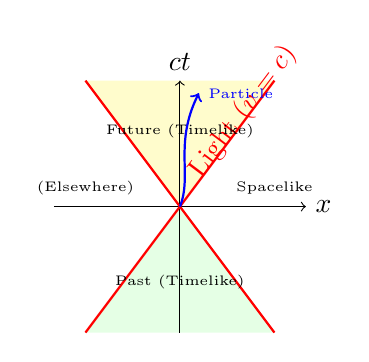
\begin{tikzpicture}[scale=0.8]
                % Light Cone
                \fill[yellow!20] (0,0) -- (-1.5,2) -- (1.5,2) -- cycle; % Future
                \fill[green!10] (0,0) -- (-1.5,-2) -- (1.5,-2) -- cycle; % Past
                
                % Axes
                \draw[->] (-2,0) -- (2,0) node[right] {$x$};
                \draw[->] (0,-2) -- (0,2) node[above] {$ct$};
                
                % Cone Lines
                \draw[thick, red] (-1.5,-2) -- (1.5,2);
                \draw[thick, red] (1.5,-2) -- (-1.5,2);
                \node[red, rotate=53] at (1.0, 1.5) {Light ($v=c$)};
                
                % Regions
                \node at (0, 1.2) {\tiny Future (Timelike)};
                \node at (0, -1.2) {\tiny Past (Timelike)};
                \node at (1.5, 0.3) {\tiny Spacelike};
                \node at (-1.5, 0.3) {\tiny (Elsewhere)};
                
                % Worldline
                \draw[thick, blue, ->] (0,0) .. controls (0.2, 0.5) and (-0.1, 1.0) .. (0.3, 1.8);
                \node[blue, right] at (0.3, 1.8) {\tiny Particle};
            \end{tikzpicture}
            
            \vspace{0.2em}
            \scriptsize{所有有质量粒子的世界线 (Worldline) 必须被“囚禁”在光锥内部 (斜率 $>1$)。}
    \end{columns}
\end{frame}

\begin{frame}[shrink=15]{进阶视点 II:四维矢量}
    \begin{columns}[T]
        \column{0.48\textwidth}
            \footnotesize
            \begin{block}{1. 定义与变换}
                将时间与空间打包为 $X^\mu = (ct, \vec{r})$。
                同理定义\textbf{四维动量} $P^\mu$:
                \begin{equation}
                    P^\mu = (E/c, \vec{p}) = (p^0, p^1, p^2, p^3)
                \end{equation}
                遵循洛伦兹变换矩阵:$P'^\mu = \Lambda^\mu_\nu P^\nu$。
            \end{block}

            \begin{block}{2. 标量积 (Scalar Product)}
                定义内积 $A \cdot B = A^0 B^0 - \vec{A} \cdot \vec{B}$。
                \textbf{关键性质}:该内积是\textbf{洛伦兹不变量}。
                $$ P \cdot P = (E/c)^2 - p^2 = \text{const} $$
            \end{block}

            \vspace{0.2em}
            \centering
            % 将图移至左侧
            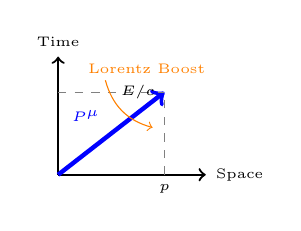
\begin{tikzpicture}[scale=0.75]
                % Axes
                \draw[->, thick] (0,0) -- (2.5,0) node[right] {\tiny Space};
                \draw[->, thick] (0,0) -- (0,2.0) node[above] {\tiny Time};
                
                % Vector
                \draw[ultra thick, blue, ->] (0,0) -- (1.8, 1.4) node[midway, above left] {\tiny $P^\mu$};
                
                % Projections
                \draw[dashed, gray] (1.8,0) -- (1.8,1.4);
                \draw[dashed, gray] (0,1.4) -- (1.8,1.4) node[left, black] {\tiny $E/c$};
                \node[below] at (1.8, 0) {\tiny $p$};
                
                % Rotation hint
                \draw[->, orange, bend right] (0.8, 1.6) to (1.6, 0.8);
                \node[orange, font=\tiny] at (1.5, 1.8) {Lorentz Boost};
            \end{tikzpicture}

        \column{0.48\textwidth}
            \small % 右栏字号可以稍大,因为只有一段话
            \begin{alertblock}{Survival Algorithm: 模长即质量}
                四维动量的模长平方就是静质量!
                \begin{equation}
                    P^2 \equiv P \cdot P = m_0^2 c^2
                \end{equation}
                
                \textbf{高阶应用:无需算出速度}
                \\ 对于碰撞 $A+B \to C+D$,直接利用四维动量守恒:
                $$ P_A + P_B = P_C + P_D $$
                两边平方(利用标量积):
                $$ (P_A + P_B)^2 = (P_C + P_D)^2 $$
                $$ P_A^2 + P_B^2 + 2P_A \cdot P_B = \dots $$
                $$ m_A^2 c^2 + m_B^2 c^2 + 2(E_A E_B/c^2 - \vec{p}_A \cdot \vec{p}_B) = \dots $$
                \textbf{结论}:这就是计算阈值能量的最快路径。
            \end{alertblock}
    \end{columns}
\end{frame}

\begin{frame}[shrink=10]{进阶视点 III:闵氏时空图}
    \begin{columns}[T]
        \column{0.48\textwidth}
            \footnotesize
            \begin{block}{1. 坐标轴的倾斜}
                洛伦兹变换可以看作坐标轴的“双曲旋转”。
                \begin{itemize}
                    \item \textbf{时间轴 $ct'$} ($x'=0$):对应方程 $x = \beta ct$。
                    \item \textbf{空间轴 $x'$} ($t'=0$):对应方程 $ct = \beta x$。
                \end{itemize}
                \textbf{结论}:动系的两个轴向\textbf{光锥}靠拢,夹角变小。
            \end{block}

            \begin{block}{2. 同时性的几何解释}
                在 $S'$ 系同时的事件位于平行于 $x'$ 轴的直线上。
                \\ 由于 $x'$ 轴是倾斜的,它切出的 $S$ 系时间 $t$ 必然不同。
                \\ $\implies$ \textbf{倾斜导致异地不同时}。
            \end{block}

        \column{0.48\textwidth}
            \centering
            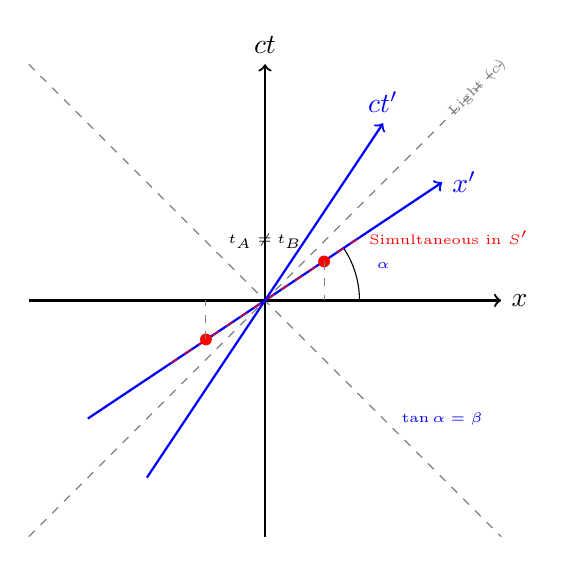
\begin{tikzpicture}[scale=1.5]
                % Light Cone
                \draw[dashed, gray] (-2,-2) -- (2,2);
                \draw[dashed, gray] (-2,2) -- (2,-2);
                \node[gray, rotate=45] at (1.8, 1.8) {\tiny Light ($c$)};
                
                % S Frame (Orthogonal)
                \draw[->, thick] (-2,0) -- (2,0) node[right] {$x$};
                \draw[->, thick] (0,-2) -- (0,2) node[above] {$ct$};
                
                % S' Frame (Skewed)
                \draw[->, thick, blue] (-1.5,-1.0) -- (1.5,1.0) node[right] {$x'$};
                \draw[->, thick, blue] (-1.0,-1.5) -- (1.0,1.5) node[above] {$ct'$};
                
                % Angle
                \draw (0.8,0) arc (0:33.7:0.8);
                \node[blue] at (1.0, 0.3) {\tiny $\alpha$};
                \node[align=left, font=\tiny, blue] at (1.5, -1.0) {$\tan \alpha = \beta$};
                
                % Event A and B (Simultaneous in S')
                \fill[red] (0.5, 0.33) circle (0.05);
                \fill[red] (-0.5, -0.33) circle (0.05);
                \draw[red, dashed] (-0.8, -0.53) -- (0.8, 0.53);
                \node[red, right] at (0.8, 0.53) {\tiny Simultaneous in $S'$};
                
                % Comparison to S
                \draw[dashed, gray] (0.5, 0.33) -- (0.5, 0);
                \draw[dashed, gray] (-0.5, -0.33) -- (-0.5, 0);
                \node[black, font=\tiny] at (0, 0.5) {$t_A \ne t_B$};
            \end{tikzpicture}
            
            \vspace{0.2em}
            \small
            \begin{alertblock}{校准双曲线 (Calibration)}
                注意:斜轴上的单位长度与正轴不同!
                $$ (ct)^2 - x^2 = \pm 1 $$
                刻度位于双曲线上,而非圆上。
            \end{alertblock}
    \end{columns}
\end{frame}

\begin{frame}[shrink=5]{进阶视点 IV:相对论质心速度}
    \begin{columns}[T]
        \column{0.48\textwidth}
            \footnotesize
            \textbf{经典 vs 相对论}
                \begin{itemize}
                    \item \textbf{经典力学}:
                    $$ \vec{v}_{cm} = \frac{\sum m_i \vec{v}_i}{\sum m_i} $$
                    \item \textbf{相对论}:质量不再守恒,能量扮演“惯性”的角色。
                    \begin{equation}
                        \vec{\beta}_{cm} = \frac{\vec{v}_{cm}}{c} = \frac{\sum \vec{p}_i c}{\sum E_i}
                    \end{equation}
                \end{itemize}
            
            \begin{exampleblock}{推导思路}
                在质心系中,总动量为零 ($\sum \vec{p}'_i = 0$)。
                利用洛伦兹变换 $P'_{tot} = \Lambda P_{tot}$,令空间分量为0,即可解出该系的相对速度 $\beta$。
            \end{exampleblock}

        \column{0.48\textwidth}
            \small
            \begin{alertblock}{Survival Application: 追及碰撞}
                \textbf{题目}:光子($E$) 追击 电子($E_e, p_e$)。求质心系速度。
                
                \textbf{直接代公式}:
                $$ \beta_{cm} = \frac{p_\gamma c + p_e c}{E_\gamma + E_e} = \frac{E + p_e c}{E + E_e} $$
                
                \textbf{检验}:
                若电子静止 ($p_e=0, E_e=mc^2$):
                $$ \beta_{cm} = \frac{E}{E + mc^2} $$
                \textit{这比先进行复杂的坐标变换要快得多!}
            \end{alertblock}
    \end{columns}
\end{frame}

\subsection{典型模型与佯谬解析}

\begin{frame}[shrink=5]{综合模型 A:车库佯谬}
    \begin{columns}[T]
        \column{0.48\textwidth}
            \footnotesize
            \begin{block}{题目场景}
                一根静止长度为 $L_0$ 的梯子,以速度 $v$ ($\gamma=2$) 飞向一个静止长度也为 $L_0$ 的车库。
                \begin{itemize}
                    \item \textbf{前门与后门}:车库有两个门,平时开着。
                    \item \textbf{操作}:当梯子完全进入车库时,两扇门\textbf{同时}快速关闭再打开。
                \end{itemize}
            \end{block}

            \begin{alertblock}{矛盾的焦点}
                \textbf{车库管理员 (Ground)}:
                \\ 梯子动了 $\implies$ 尺缩效应。
                $$ L_{lad} = L_0 / \gamma = 0.5 L_0 < L_{gar} $$
                \textbf{结论}:梯子变短了,\textbf{能装下}!门可以同时关。
            \end{alertblock}

        \column{0.48\textwidth}
            \footnotesize
            \begin{alertblock}{梯子观测者 (Ladder)}
                \textbf{相对性原理}:
                \\ 梯子不动,车库在动 $\implies$ 车库尺缩。
                $$ L'_{gar} = L_0 / \gamma = 0.5 L_0 < L_{lad} $$
                \textbf{结论}:车库变短了,梯子比车库长一倍,\textbf{绝对装不下}!
                \\ 门怎么可能同时关上而不夹断梯子?
            \end{alertblock}

            \vspace{0.5em}
            \centering
            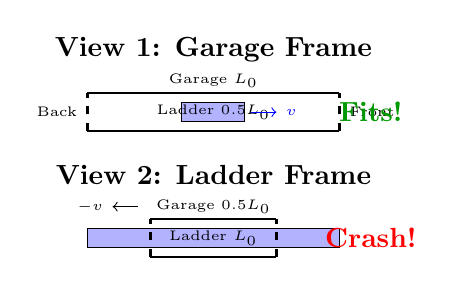
\begin{tikzpicture}[scale=0.8]
                % Garage Frame
                \node at (0, 2.5) {\textbf{View 1: Garage Frame}};
                \draw[thick] (-2, 1.8) -- (2, 1.8); % Roof
                \draw[thick] (-2, 1.2) -- (2, 1.2); % Floor
                \draw[thick, dashed] (-2, 1.2) -- (-2, 1.8) node[midway, left]{\tiny Back};
                \draw[thick, dashed] (2, 1.2) -- (2, 1.8) node[midway, right]{\tiny Front};
                \node at (0, 2.0) {\tiny Garage $L_0$};
                
                \draw[fill=blue!30] (-0.5, 1.35) rectangle (0.5, 1.65);
                \node at (0, 1.5) {\tiny Ladder $0.5L_0$};
                \draw[->, blue] (0.6, 1.5) -- (1.0, 1.5) node[right]{\tiny $v$};
                \node[green!60!black, font=\bfseries] at (2.5, 1.5) {Fits!};

                % Ladder Frame
                \node at (0, 0.5) {\textbf{View 2: Ladder Frame}};
                \draw[fill=blue!30] (-2, -0.65) rectangle (2, -0.35);
                \node at (0, -0.5) {\tiny Ladder $L_0$};
                
                \draw[thick] (-1, -0.2) -- (1, -0.2); 
                \draw[thick] (-1, -0.8) -- (1, -0.8);
                \draw[thick, dashed] (-1, -0.8) -- (-1, -0.2);
                \draw[thick, dashed] (1, -0.8) -- (1, -0.2);
                \node at (0, 0) {\tiny Garage $0.5L_0$};
                \draw[->] (-1.2, 0) -- (-1.6, 0) node[left]{\tiny $-v$};
                \node[red, font=\bfseries] at (2.5, -0.5) {Crash!};
            \end{tikzpicture}
    \end{columns}
\end{frame}

\begin{frame}[shrink=20]{综合模型 A:车库佯谬}
    \begin{columns}[T]
        \column{0.48\textwidth}
            \footnotesize
            \begin{block}{破解钥匙:同时的相对性}
                “装得下”的定义是:梯子头碰到前门(Event A) 与 梯子尾离开后门(Event B) \textbf{同时发生}。
                \begin{itemize}
                    \item 在车库系:$\Delta t = t_A - t_B = 0$ (同时)。
                    \item 在梯子系:$\Delta t' \neq 0$!
                \end{itemize}
            \end{block}
            
            \begin{exampleblock}{梯子系的剧本 (Calculated)}
                利用变换 $\Delta t' = \gamma(\Delta t - v\Delta x/c^2)$:
                \\ 设车库系两门距离 $\Delta x = L_0$。
                $$ \Delta t' = -\gamma \frac{v}{c^2} L_0 < 0 $$
                \textbf{含义}:$t'_A < t'_B$。即\textbf{前门先关},后门\textbf{后关}。
            \end{exampleblock}

        \column{0.48\textwidth}
            \small
            \begin{alertblock}{真相:时间差救了梯子}
                在梯子看来,前门先关上,\textbf{然后马上打开},让梯子头出去;
                \\ 过了很久之后,后门才关上。
                \\ $\implies$ 梯子从未“同时”被关在里面,但也没有被门夹断。
            \end{alertblock}

            \vspace{0.5em}
            \centering
            % 梯子系的时空图
            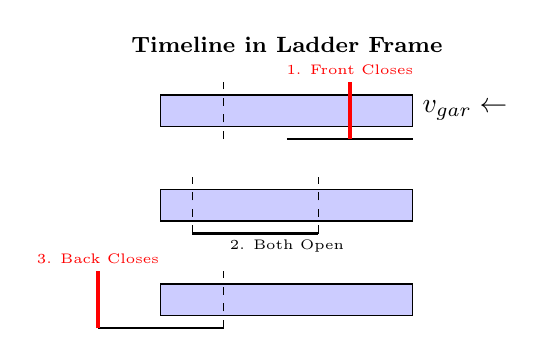
\begin{tikzpicture}[scale=0.8]
                \node at (0, 2.8) {\footnotesize \textbf{Timeline in Ladder Frame}};
                
                % Step 1: Front Door
                \draw[fill=blue!20] (-2, 1.5) rectangle (2, 2.0); % Ladder
                \draw[thick] (0, 1.3) -- (2, 1.3); % Garage floor
                \draw[ultra thick, red] (1.0, 1.3) -- (1.0, 2.2); % Front Door Closed
                \node[red, font=\tiny] at (1.0, 2.4) {1. Front Closes};
                \draw[dashed] (-1.0, 1.3) -- (-1.0, 2.2); % Back Door Open
                \node[right] at (2.0, 1.75) {$v_{gar} \leftarrow$};
                
                % Step 2: Middle
                \draw[fill=blue!20] (-2, 0) rectangle (2, 0.5);
                \draw[thick] (-1.5, -0.2) -- (0.5, -0.2); % Garage moved left
                \draw[dashed] (0.5, -0.2) -- (0.5, 0.7); % Front Open
                \draw[dashed] (-1.5, -0.2) -- (-1.5, 0.7); % Back Open
                \node[font=\tiny] at (0, -0.4) {2. Both Open};
                
                % Step 3: Back Door
                \draw[fill=blue!20] (-2, -1.5) rectangle (2, -1.0);
                \draw[thick] (-3.0, -1.7) -- (-1.0, -1.7); % Garage further left
                \draw[dashed] (-1.0, -1.7) -- (-1.0, -0.8); % Front Open
                \draw[ultra thick, red] (-3.0, -1.7) -- (-3.0, -0.8); % Back Door Closed
                \node[red, font=\tiny] at (-3.0, -0.6) {3. Back Closes};
            \end{tikzpicture}
            
            \vspace{0.2em}
            \scriptsize{\textbf{结论}:两系对于“物理事实”(梯子没断)是一致的,只是对“同时”的描述不同。}
    \end{columns}
\end{frame}

\begin{frame}[shrink=15]{综合模型 B:孪生子佯谬}
    \begin{columns}[T]
        \column{0.48\textwidth}
            \footnotesize
            \begin{block}{场景描述}
                双胞胎兄弟,哥哥 A 留在地球,弟弟 B 乘坐飞船去旅行。
                \begin{itemize}
                    \item \textbf{去程}:B 以 $v$ 飞往 $\Delta x$ 外的星球。
                    \item \textbf{返程}:B 到达后立即反向,以 $-v$ 飞回地球。
                \end{itemize}
            \end{block}

            \begin{alertblock}{佯谬逻辑 (The "Paradox")}
                \begin{itemize}
                    \item \textbf{A 的视角}:B 在动,B 的钟变慢。结论:\textbf{B 比 A 年轻}。
                    \item \textbf{B 的视角}:A 在动(相对向后退),A 的钟变慢。结论:\textbf{A 比 B 年轻}。
                \end{itemize}
                当 B 回到地球时,两人面对面比年龄,不可能既是“A老”又是“B老”。\alert{谁错了?}
            \end{alertblock}

        \column{0.48\textwidth}
            \centering
            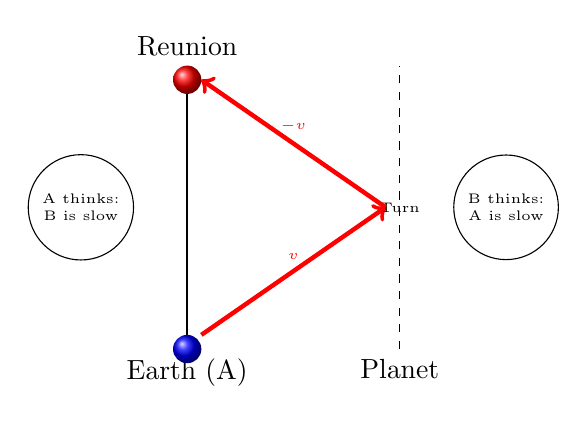
\begin{tikzpicture}[scale=0.9]
                % Earth A
                \draw[thick] (0, -2) -- (0, 2);
                \node[below] at (0, -2) {Earth (A)};
                \shade[ball color=blue] (0, -2) circle (0.2);
    
                % Planet
                \draw[dashed] (3, -2) -- (3, 2);
                \node[below] at (3, -2) {Planet};
    
                % Path of B
                \draw[->, ultra thick, red] (0.2, -1.8) -- (2.8, 0) node[midway, above]{\tiny $v$};
                \node at (3, 0) {\tiny Turn};
                \draw[->, ultra thick, red] (2.8, 0) -- (0.2, 1.8) node[midway, above]{\tiny $-v$};
                \shade[ball color=red] (0, 1.8) circle (0.2);
                \node[above] at (0, 2) {Reunion};
    
                % Comparison bubbles
                % 【修复点】加上了 align=center
                \node[draw, circle, fill=white, font=\tiny, align=center] at (-1.5, 0) {A thinks:\\B is slow};
                \node[draw, circle, fill=white, font=\tiny, align=center] at (4.5, 0) {B thinks:\\A is slow};
            \end{tikzpicture}

            \vspace{0.5em}
            \footnotesize
            \begin{block}{错误的根源}
                相对论只适用于\textbf{惯性系}。
                \\ A 始终在地球(近似惯性系)。
                \\ B \alert{必须减速并掉头},经历了巨大的\textbf{加速度},换了参考系。
                \\ $\implies$ A 和 B 的地位\textbf{不对称}!
            \end{block}
    \end{columns}
\end{frame}

\begin{frame}[shrink=20]{综合模型 B:孪生子佯谬}
    \begin{columns}[T]
        \column{0.48\textwidth}
            \footnotesize
            \begin{block}{1. 世界线长度法 (最佳解法)}
                人经历的苍老程度取决于他手表的读数(固有时 $\tau$)。
                $$ \tau = \int d\tau = \int \sqrt{1 - v(t)^2/c^2} dt $$
                \begin{itemize}
                    \item \textbf{哥哥 A}:$v=0$。
                    $$ \tau_A = \int_0^T 1 dt = T $$
                    \item \textbf{弟弟 B}:$v \neq 0$。
                    $$ \tau_B = \int_0^T \sqrt{1-\beta^2} dt = T/\gamma $$
                \end{itemize}
                \textbf{结论}:$\tau_B < \tau_A$,旅行回来的弟弟\textbf{确实更年轻}。
            \end{block}

        \column{0.48\textwidth}
            \small
            \begin{alertblock}{2. 闵氏几何三角形不等式}
                在欧氏几何中,两点之间直线最短。
                \\ 在闵氏时空中,两点之间\textbf{直线最长}(固有时最大)!
                \begin{equation}
                    \tau_{\text{straight}} > \tau_{\text{bent}}
                \end{equation}
                A 走的是直线(惯性),B 走的是折线(加速)。
            \end{alertblock}

            \vspace{0.5em}
            \centering
            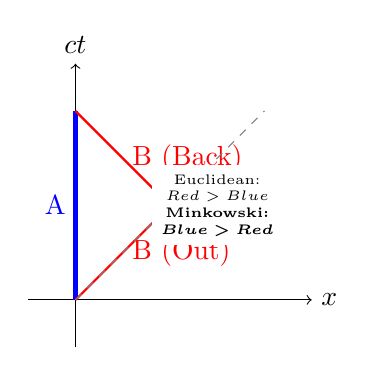
\begin{tikzpicture}[scale=1.2]
                % Axes
                \draw[->] (-0.5,0) -- (2.5,0) node[right] {$x$};
                \draw[->] (0,-0.5) -- (0,2.5) node[above] {$ct$};
                
                % A's Worldline (Straight)
                \draw[ultra thick, blue] (0,0) -- (0,2.0);
                \node[blue, left] at (0, 1.0) {A};
                
                % B's Worldline (Bent)
                \draw[thick, red] (0,0) -- (1.0, 1.0) -- (0, 2.0);
                \node[red, right] at (0.5, 0.5) {B (Out)};
                \node[red, right] at (0.5, 1.5) {B (Back)};
                
                % Light Cone
                \draw[dashed, gray] (0,0) -- (2,2);
                
                % Comparison
                \node[font=\tiny, align=center, fill=white] at (1.5, 1.0) {
                    Euclidean:\\
                    $Red > Blue$\\
                    \textbf{Minkowski:}\\
                    $\bm{Blue > Red}$
                };
            \end{tikzpicture}

            \vspace{0.2em}
            \scriptsize{注意:B 在掉头瞬间,从一个惯性系跳到另一个,这里的“跳跃”导致了时间的缺失。}
    \end{columns}
\end{frame}

\subsection{尺缩钟慢解题核心算法}

\begin{frame}[shrink=5]{核心判定:如何精准锁定“本征量”?}
    \begin{columns}[T]
        \column{0.48\textwidth}
            \footnotesize
            \begin{block}{1. 判定固有时 (Proper Time) $\Delta \tau$}
                \textbf{算法:数钟法}
                \begin{itemize}
                    \item 若某个观测者只用\textbf{一只钟}(就在他手腕上)就测出了两个事件的间隔,则他测得的一定是 $\Delta \tau$。
                    \item 固有时 $\Delta \tau$ 是所有观测者中测得时间间隔\textbf{最小}的。
                    \item \textit{公式}:$\Delta t_{others} = \gamma \Delta \tau$
                \end{itemize}
            \end{block}

            \begin{block}{2. 判定原长 (Proper Length) $L_0$}
                \textbf{算法:相对静止法}
                \begin{itemize}
                    \item 若测量者与被测物体\textbf{相对静止},则他测得的是 $L_0$。
                    \item 原长 $L_0$ 是所有观测者中测得长度\textbf{最大}的。
                    \item \textit{公式}:$L_{moving} = L_0 / \gamma$
                \end{itemize}
            \end{block}

        \column{0.48\textwidth}
            \small
            \begin{alertblock}{解题陷阱:千万不要交叉混用}
                \begin{itemize}
                    \item \textbf{错误做法}:先算尺缩再算钟慢,逻辑极易打架。
                    \item \textbf{正确姿势}:
                        \begin{enumerate}
                            \item 选定一个参考系。
                            \item 只对这个系下的物理量套用效应。
                            \item \textbf{终极大法}:如果分不清谁缩谁慢,直接列\textbf{洛伦兹变换}坐标方程。
                        \end{enumerate}
                \end{itemize}
            \end{alertblock}

            \vspace{0.5em}
            \centering
            \begin{tikzpicture}[scale=0.8, every node/.style={transform shape}]
                \node[draw, thick, rounded corners, fill=orange!10, inner sep=6pt] {
                    \begin{tabular}{c}
                        \textbf{解题口诀}\\
                        一只钟测 $\Delta \tau$,静止系里量 $L_0$\\
                        运动系看时间长,运动系量长度短
                    \end{tabular}
                };
            \end{tikzpicture}
    \end{columns}
\end{frame}

\begin{frame}[shrink=5]{万能算法:洛伦兹坐标变换“三步走”}
    \begin{columns}[T]
        \column{0.5\textwidth}
            \footnotesize
            \begin{enumerate}
                \item \textbf{第一步:定事件点 (Events)}
                \\ 将题目描述转化为两个具体的时空点:
                \\ 事件 A:$(x_A, t_A)$;事件 B:$(x_B, t_B)$。
                
                \item \textbf{第二步:定相对速度 ($v$)}
                \\ 确定 $S'$ 系相对于 $S$ 系的速度。
                \\ \alert{\textbf{注意:}} 向左运动 $v < 0$,向右运动 $v > 0$。
                
                \item \textbf{第三步:套差分公式 ($\Delta$)}
                \\ 考试中求“间隔”的情况远多于求“单点坐标”:
                \begin{equation}
                    \begin{aligned}[box=\fbox]{align*}
                        \Delta x' &= \gamma (\Delta x - v \Delta t) \\
                        \Delta t' &= \gamma (\Delta t - \frac{v}{c^2} \Delta x)
                    \end{aligned}
                \end{equation}
            \end{enumerate}

        \column{0.45\textwidth}
            \small
            \begin{exampleblock}{算法演示:同时的相对性}
                地面 $S$ 同时闪光 ($\Delta t=0$),间隔 $L$。飞船 $S'$ 测得时间间隔?
                \\ \textbf{带入算法:}
                \begin{itemize}
                    \item $\Delta t = 0$, $\Delta x = L$
                    \item $\Delta t' = \gamma (0 - \frac{v L}{c^2}) = -\frac{\gamma v L}{c^2}$
                \end{itemize}
                \textbf{结果分析:}
                \\ $\Delta t' < 0$ 说明在 $S'$ 系中,$x$ 较大的事件(前方)先发生。这就是“后方先发”判据的数学推导。
            \end{exampleblock}
            
            \vspace{0.5em}
            \centering
            \begin{tikzpicture}
                \node[fill=red!5, draw=red!50, dashed, inner sep=5pt] {
                    \scriptsize \textbf{技巧:} 计算中尽量保留 $c$ 和 $\beta$,直到最后一步。
                };
            \end{tikzpicture}
    \end{columns}
\end{frame}

\section{作业习题讲解}

\begin{frame}
    \begin{center}
        {\Huge 作业习题讲解}
    \end{center}
\end{frame}

\section{Q\&A}

\begin{frame}
    \begin{center}
        {\Huge\calligra Q\&A}
    \end{center}
\end{frame}

\begin{frame}
    \begin{center}
        {\Huge\calligra Thanks!}
    \end{center}
\end{frame}

\end{document}